\documentclass[a4paper,10pt]{report}
\usepackage{mathptmx}

\usepackage{tabularx} % extra features for tabular environment
\usepackage{amsmath}  % improve math presentation
% \usepackage{float}
% \usepackage{pdfpages}


\usepackage{graphicx} % takes care of graphic including machinery
\graphicspath{ {./figures/} }
%\usepackage[margin=1in,letterpaper]{geometry} % decreases margins
%\usepackage{cite} % takes care of citations
\usepackage[final]{hyperref} % adds hyper links inside the generated pdf file
\hypersetup{
	colorlinks=true,       % false: boxed links; true: colored links
	linkcolor=blue,        % color of internal links
	citecolor=blue,        % color of links to bibliography
	filecolor=magenta,     % color of file links
	urlcolor =blue         
}
\usepackage[margin = 1in,headsep=0.5cm,headheight=2cm,letterpaper]{geometry} 

\usepackage{fancyhdr}
\pagestyle{fancy}
\lhead{Student 1 : Ahmet Akman 2442366 \\ Student 2: Kaan Demirkoparan }
\rhead{Date: \today \\ Group: Friday Morning - 6} 
%\cfoot{center of the footer!}
%\renewcommand{\headrulewidth}{0.1pt}


\begin{document}
\thispagestyle{empty}

\title{  Fall 2022 EE Project Work  \protect\\ Preliminary Report}
\author{ Ahmet Akman 2442366 \protect\\ Kaan Demirkoparan}
\date{}
\maketitle
%\tableofcontents
%\begin{abstract}
%abstract
%\end{abstract}
\section{Introduction}
In this document, the Preliminary report of the term project of the EE214 course will be presented. 
\section{General Structure and Design Philisophy}
\begin{figure}[h]
    \centering
    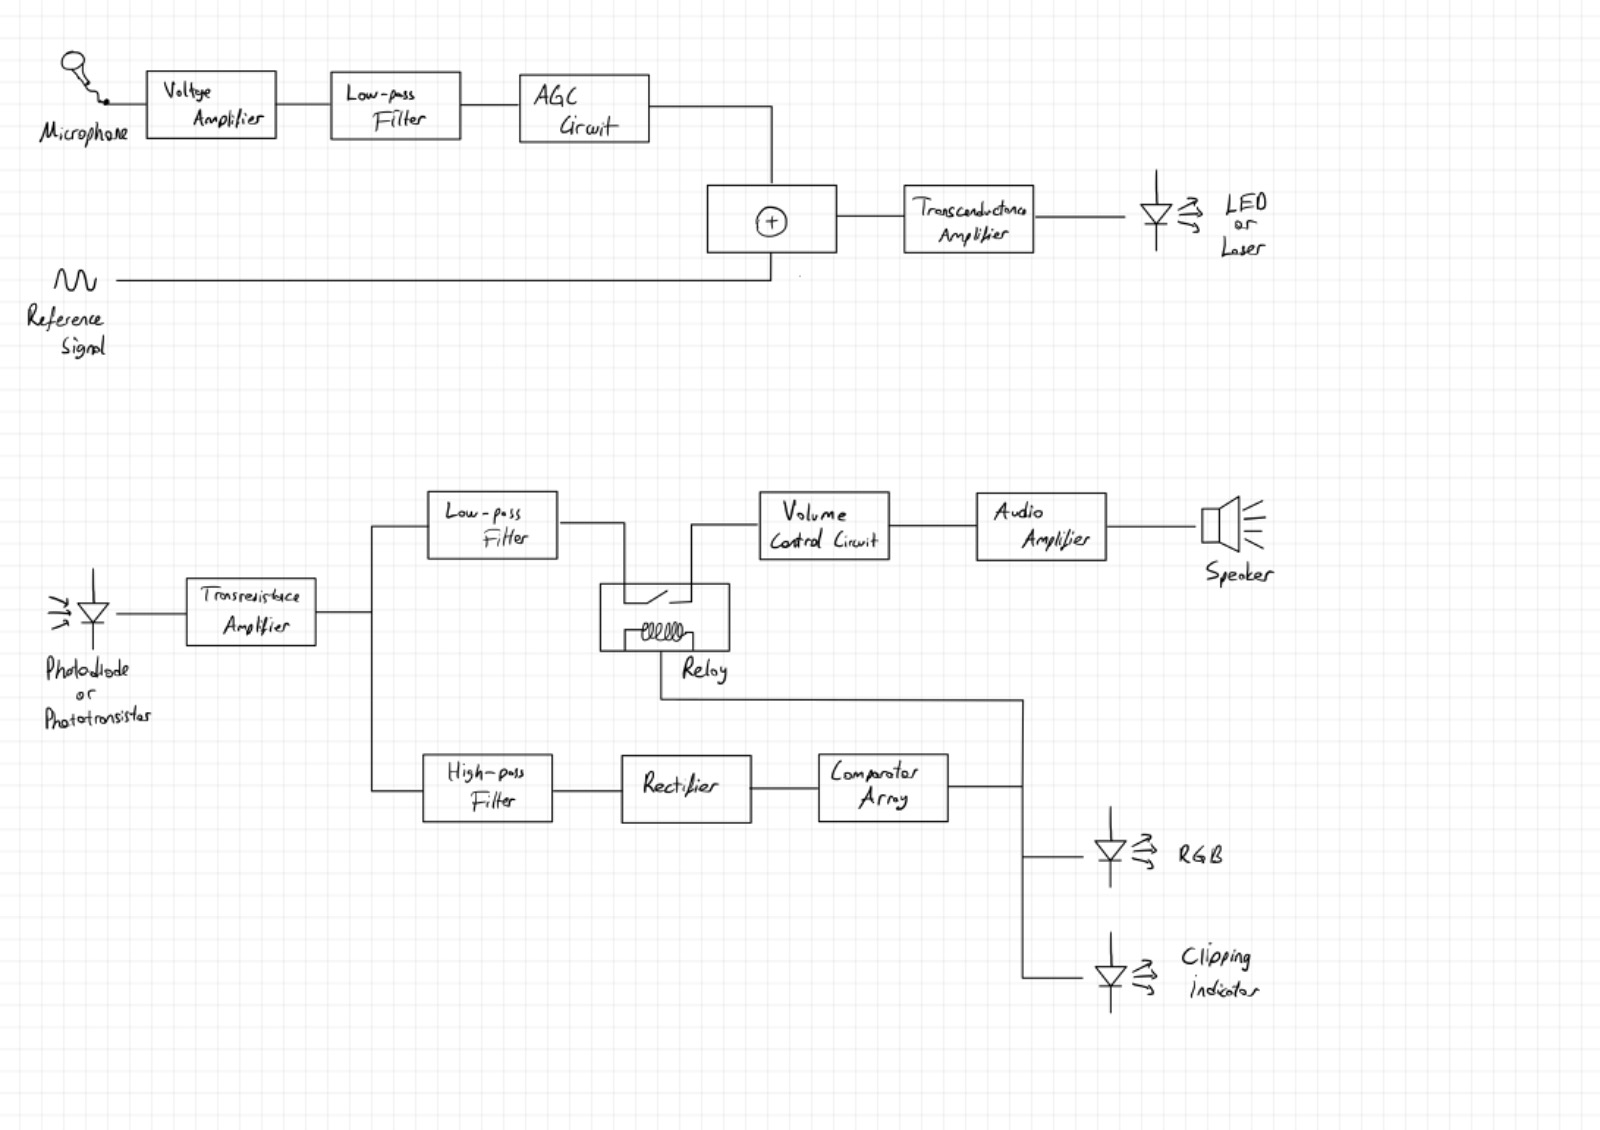
\includegraphics[width = 1\textwidth]{general_structure.jpeg}
    \caption{General Structure}
\end{figure} 
Deneme
Deneme 123 Deneme 123
abc 
abc

\section{Transmitter Side}
\subsection{Input and Early Stage Amplification}
\subsection{Automatic Gain Control}
\subsection{Light Transmitter}
\section{Receiver Side}
\subsection{Light Receiver}
\subsection{Demodulation and Speker Side}
\subsection{Signal Quality Indication}

\section{Conclusion}
In this document, the Preliminary report of the term project of the EE313 course is presented. 

\end{document}

%%%%%%%%%%%%%%%%%%%%%%   EXAMPLE TABLE   %%%%%%%%%%%%%%%%%%%%%%%%%%%%%%%%
\begin{table}[H]
\begin{center}
    \caption{Resistance reading by color code convention.}
    \vspace{2mm}
    \begin{tabular}{||c | c | c||} 
        \hline
        Color Order & Value & Tolerance \\ [0.5ex] 
        \hline\hline
        Brown / Black / Red / Gold & 1k\( \Omega \) & \( \% \) 5  \\ 
        \hline
        Yellow / Violet / Red / Gold & 4.7k\( \Omega \) & \( \% \) 5   \\
        \hline
        Brown / Grey / Orange / Gold & 18k\( \Omega \) & \( \% \) 5  \\ [1ex] 
        \hline
    \end{tabular}
\end{center}
\end{table}


%%%%%%%%%%%%%%%%%%%%%%   EXAMPLE IMAGE   %%%%%%%%%%%%%%%%%%%%%%%%%%%%%%%%
\begin{figure}[H]
\centering
\includegraphics[width = 0.75\textwidth]{5.png}
\caption{Circuit schematic for the step 5}
\end{figure} 

%%%%%%%%%%%%%%%%%%%%%%   EXAMPLE IMAGE FROM PDF   %%%%%%%%%%%%%%%%%%%%%%%%%%%%%%%%
\begin{figure}[H] \centering{
	\includegraphics[scale=0.25]{2a_plot.pdf}}
	\caption{Experiment 2}
\end{figure}
%%%%%%%%%%%%%%%% Deneme Push